\chapter{DuckieTown}

\section{Umgebung}

In einer DuckieTown-Umgebung wird die Umwelt für einen DuckieBot definiert. Ein DuckieBot kann diese Umgebung dann observieren und sich in dieser bewegen. Eine DuckieTown-Umgebung wird dabei aus verschiedenen Kacheln und Objekten aufgebaut. 

\begin{figure}[H]
	\centering
	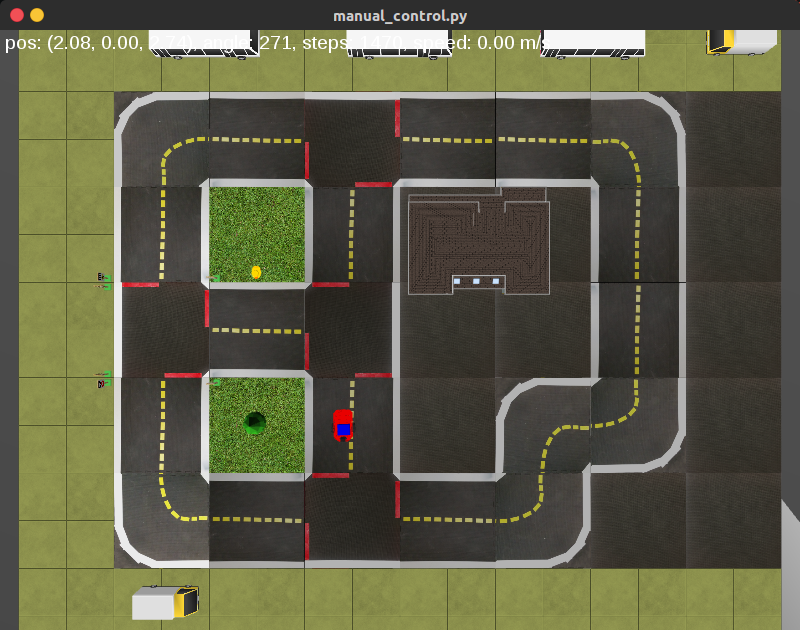
\includegraphics[width=0.6\textwidth]{kapitel2/images/duckietown-umgebung.png}
	\label{fig:duckietown-umgebung}
	\caption{Darstellung einer beispielhaften DuckieTown-Umgebung}
	\vspace{0.2cm}
	\quelle\url{https://user-images.githubusercontent.com/10503729/45590954-c88c7c00-b912-11e8-9209-f72924684e21.gif}
\end{figure}

Bei den Kacheln wird zwischen befahrbaren und nicht befahrbaren Kacheln unterschieden, wobei folgende Kacheln standardmäßig zur Verfügung stehen:

\begin{itemize}
	\item 
		\begin{tabular}[t]{lll}
			\textbf{Leere Kachel} & (nicht befahrbar) & \hspace{2.45cm} 
			$ \begin{array}{l}
				\setlength{\fboxsep}{0pt}
				\fbox{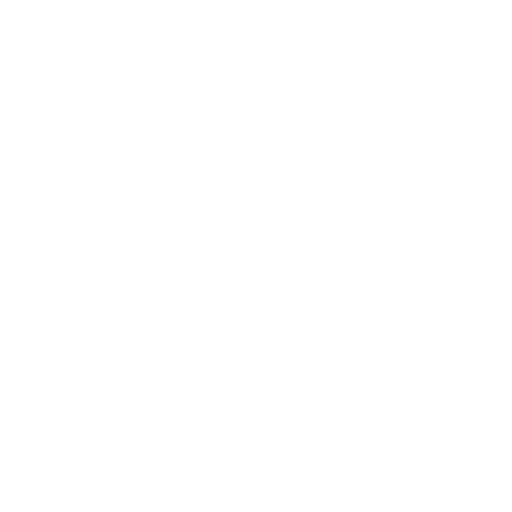
\includegraphics[scale=0.135]{kapitel2/images/empty.png}}
			\end{array} $
		\end{tabular} 
	
	\item 
		\begin{tabular}[t]{lll}
			\textbf{Gerader Streckenabschnitt} & (befahrbar) & \hspace{0.8cm}
			$ \begin{array}{l}
				\setlength{\fboxsep}{0pt}
				\fbox{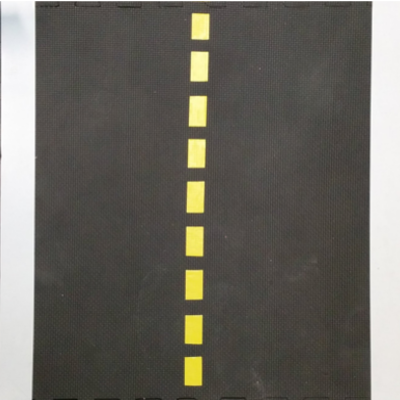
\includegraphics[scale=0.17]{kapitel2/images/straight.png}}
		  	\end{array} $
		\end{tabular}
	
	\newpage
	
	\item 
		\begin{tabular}[t]{lll}
			\textbf{Linkskurve} & (befahrbar) & \hspace{3.85cm}
			$ \begin{array}{l}
				\setlength{\fboxsep}{0pt}
				\fbox{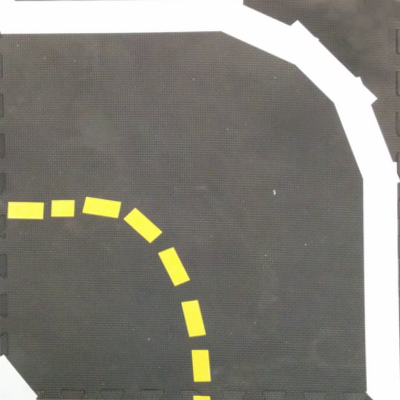
\includegraphics[scale=0.17]{kapitel2/images/left.png}}
			\end{array} $
		\end{tabular}
	
	\item 
		\begin{tabular}[t]{lll}
			\textbf{Rechtskurve} & (befahrbar) & \hspace{3.55cm}
			$ \begin{array}{l}
				\setlength{\fboxsep}{0pt}
				\fbox{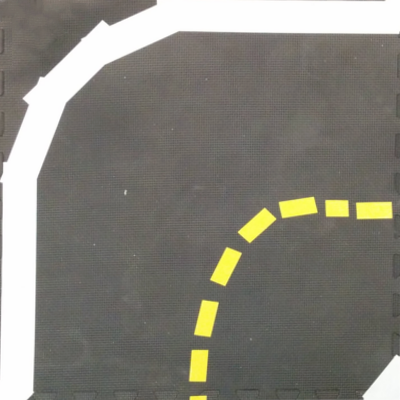
\includegraphics[scale=0.17]{kapitel2/images/right.png}}
			\end{array} $
		\end{tabular}
	
	\item 
		\begin{tabular}[t]{lll}
			\textbf{3-Wege Kreuzung} & (befahrbar) & \hspace{2.5cm}
			$ \begin{array}{l}
				\setlength{\fboxsep}{0pt}
				\fbox{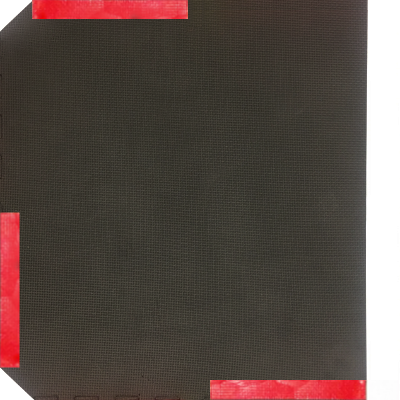
\includegraphics[scale=0.17]{kapitel2/images/3way.png}}
			\end{array} $
		\end{tabular}
	
	\item 
		\begin{tabular}[t]{lll}
			\textbf{4-Wege Kreuzung} & (befahrbar) & \hspace{2.5cm}
			$ \begin{array}{l}
				\setlength{\fboxsep}{0pt}
				\fbox{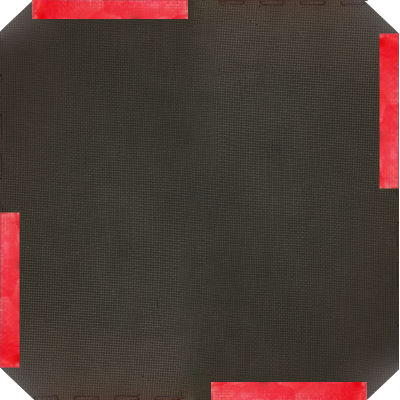
\includegraphics[scale=0.17]{kapitel2/images/4way.png}}
			\end{array} $
		\end{tabular}
	\item 
		\begin{tabular}[t]{lll}
			\textbf{Asphaltkachel} & (nicht befahrbar) & \hspace{2.25cm}
			$ \begin{array}{l}
				\setlength{\fboxsep}{0pt}
				\fbox{
\includegraphics[scale=0.17]{kapitel2/images/asphalt.png}}
			\end{array} $
		\end{tabular}
	
	\item 
		\begin{tabular}[t]{lll}
			\textbf{Graskachel} & (nicht befahrbar) & \hspace{2.85cm}
			$ \begin{array}{l}
				\setlength{\fboxsep}{0pt}
				\fbox{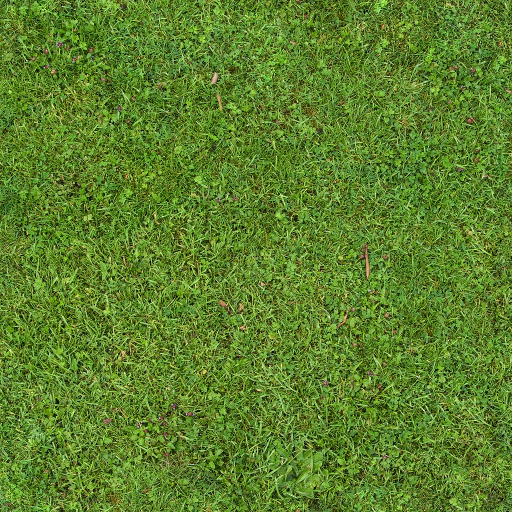
\includegraphics[scale=0.132]{kapitel2/images/grass.png}}
			\end{array} $ \\
		\end{tabular}
	
	\item 
		\begin{tabular}[t]{lll}
			\textbf{Bodenkachel} & (nicht befahrbar) & \hspace{2.55cm}
			$ \begin{array}{l}
				\setlength{\fboxsep}{0pt}
				\fbox{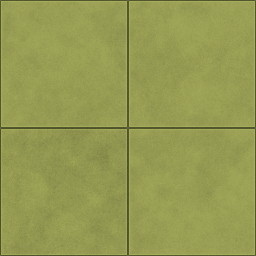
\includegraphics[scale=0.26]{kapitel2/images/floor.png}}
			\end{array} $
		\end{tabular}
\end{itemize}

Objekte sind ebenfalls nicht befahrbar und befinden sich in der Regel außerhalb des Streckenverlaufes. Es werden standardmäßig eine Vielzahl von Objekten zur Verfügung gestellt, wie zum Beispiel:

\newpage

\begin{itemize}
	\item \textbf{Haus}
	\item \textbf{Baum}
	\item \textbf{Bus}
	\item \textbf{Verkehrsschilder etc.}
\end{itemize}

Eine DuckieTown-Umgebung wird hierbei in einer \texttt{.yaml}-Datei definiert, die dann vom Simulator geladen und dargestellt wird.

\hspace{1cm}
\begin{minipage}{.73\linewidth}
	\begin{lstlisting}[caption={Beispieldefinition einer DuckieTown-Umgebung}]
		# 3x3 tiles with left turns at the corners
		# going in a counter-clockwise loop
	
		tiles:
		- [curve_left/W , straight/W, curve_left/N]
		- [straight/S   , asphalt   , straight/N]
		- [curve_left/S , straight/E, curve_left/E]
	
		tile_size: 1
	\end{lstlisting}
\end{minipage}

\section{DuckieBot}
\label{duckiebot}

Ein \href{https://get.duckietown.com/products/duckiebot-db18}{DuckieBot} ist ein kleiner mobiler Roboter mit Differenzialantrieb, der seine Umgebung über eine Kamera wahrnehmen kann. Er ist mit einem \href{https://www.raspberrypi.org/}{Raspberry Pi} ausgestattet, welcher für Berechnungen und die Datenverarbeitung zuständig ist. Die  Räder werden über Gleichstrommotoren angetrieben. Mittels eines Steuerbefehls (bestehend aus Geschwindigkeit und Richtungsänderung) kann ein DuckieBot in einer Umgebung navigiert werden. \cite{duckietown_platform}
Der Simulator ist dabei in der Lage einen solchen DuckieBot zu simulieren.

\begin{figure}[H]
	\centering
	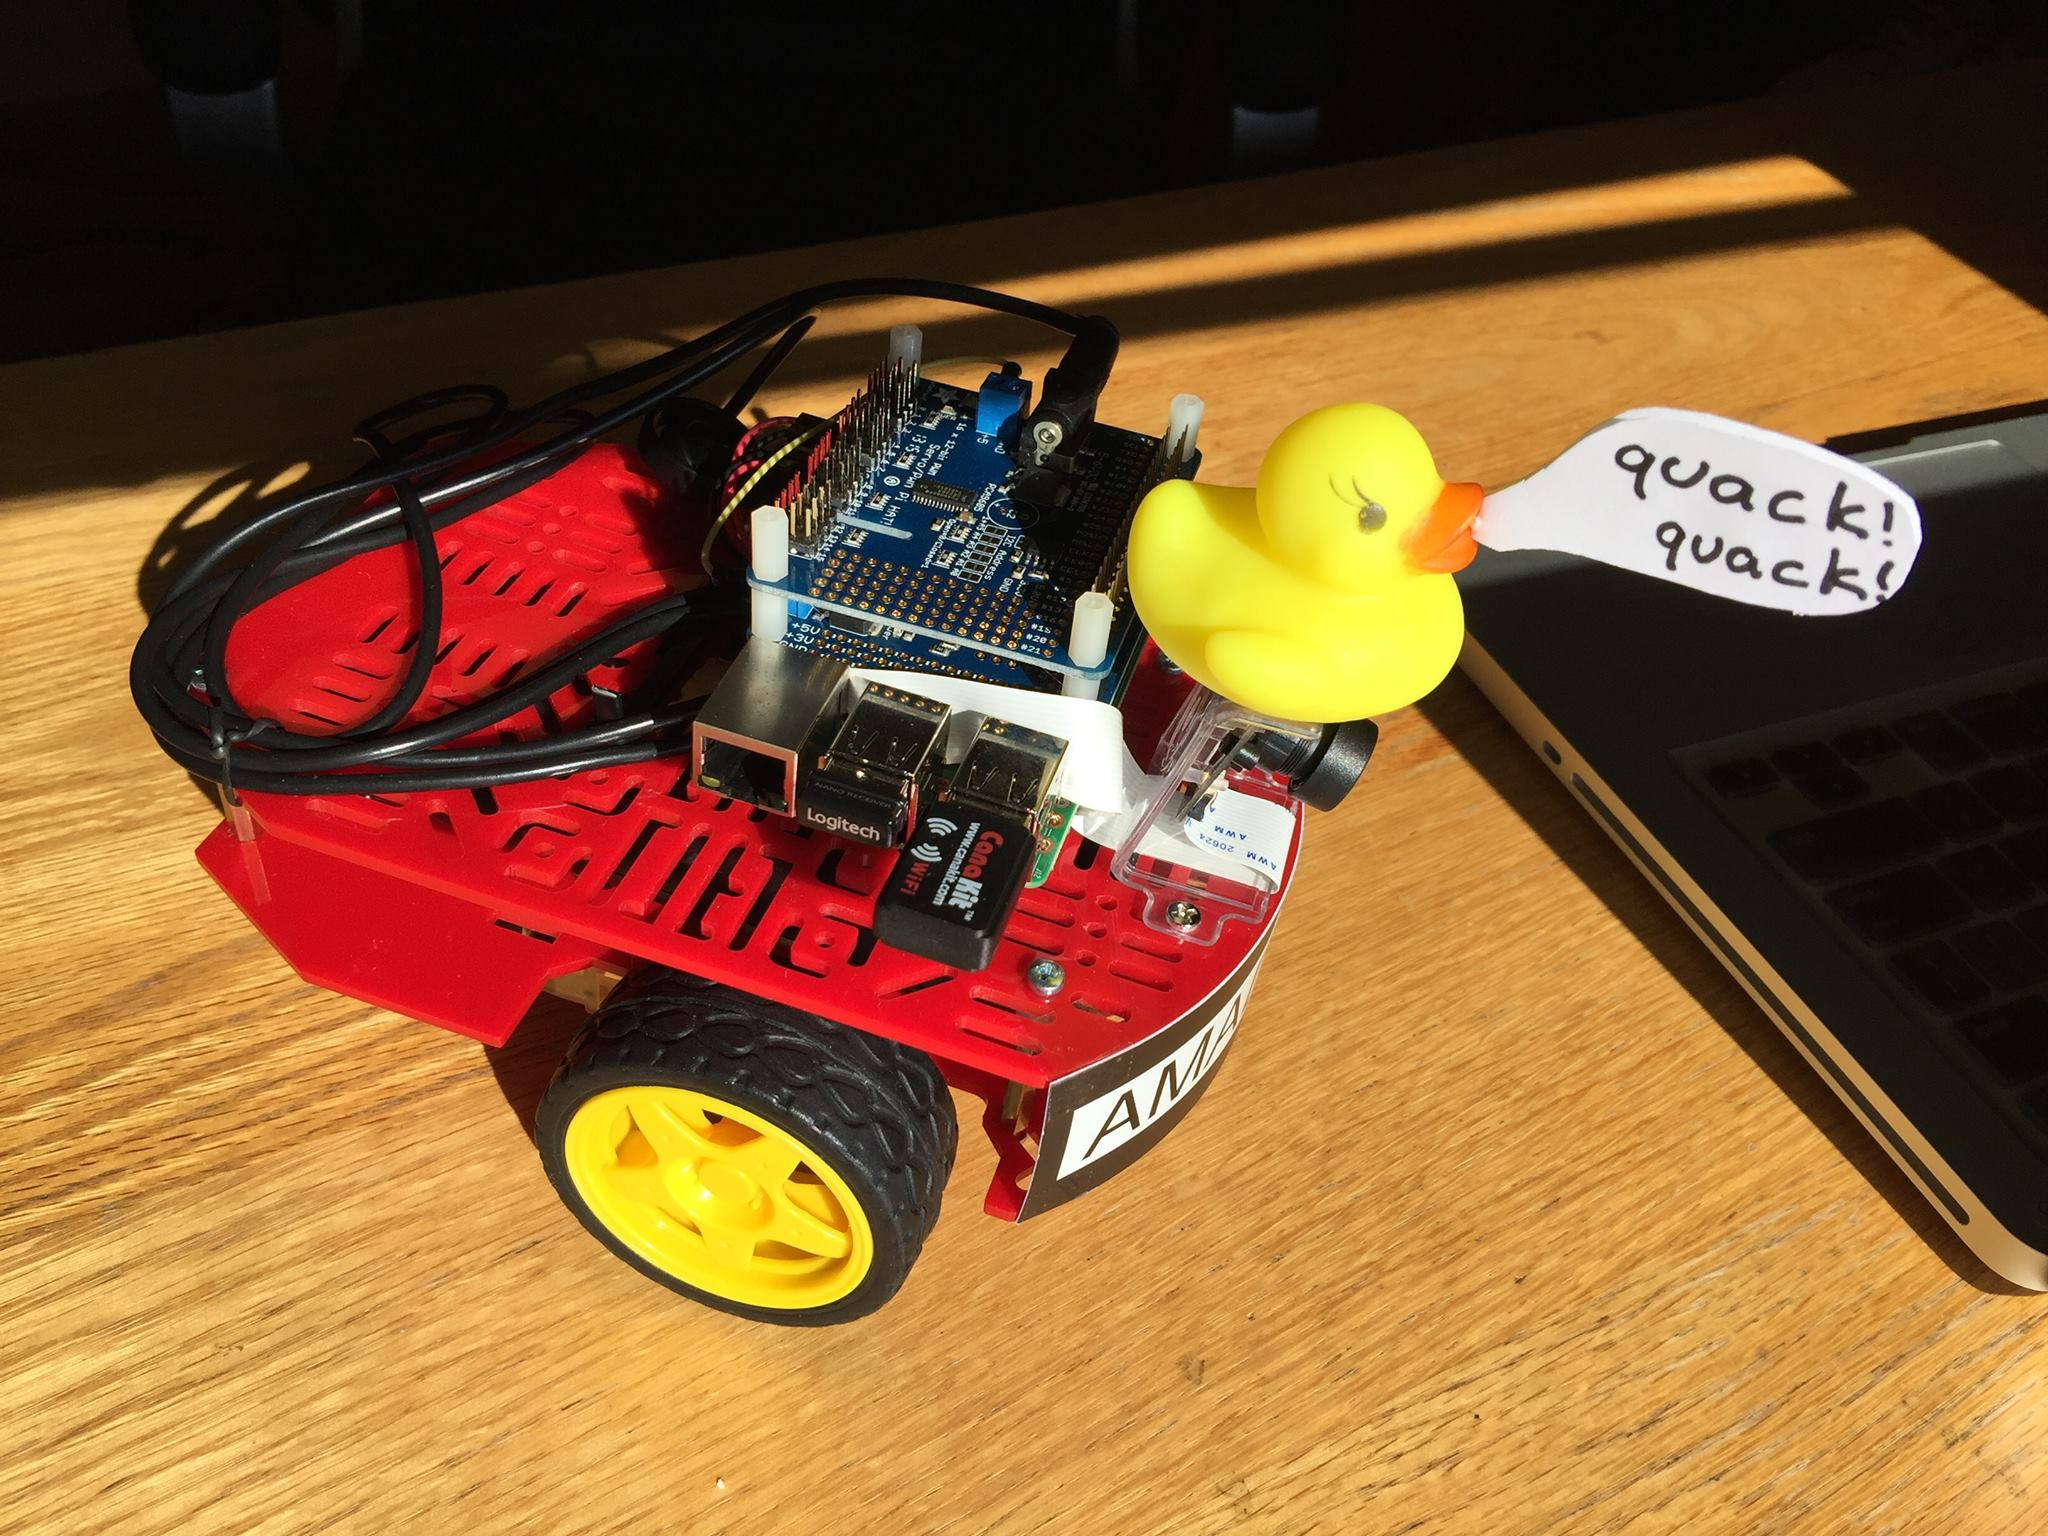
\includegraphics[width=0.385\textwidth]{kapitel2/images/duckiebot.jpg}
	\label{fig:duckiebot}
	\caption{Darstellung eines DuckieBots}
	\vspace{0.2cm}
	\quelle\url{https://cdn-blog.adafruit.com/uploads/2016/05/mercedes.jpg}
\end{figure}


\section{Simulator}

Der \href{https://github.com/duckietown/gym-duckietown}{DuckieTown-Simulator} ist ein in \href{https://www.python.org/}{\texttt{Python}} und \href{https://www.opengl.org/}{\texttt{OpenGL}} \acf{bzw} \href{http://pyglet.org/}{\texttt{Pyglet}} geschriebener Simulator für das \glqq DuckieTown-Universum\grqq. Der Simulator bietet die Möglichkeit DuckieBots (Agenten) in einer beliebigen DuckieTown-Umgebung zu platzieren und die Agenten darin zu navigieren. \cite{gym_duckietown} \\

\begin{figure}[H]
	\centering
	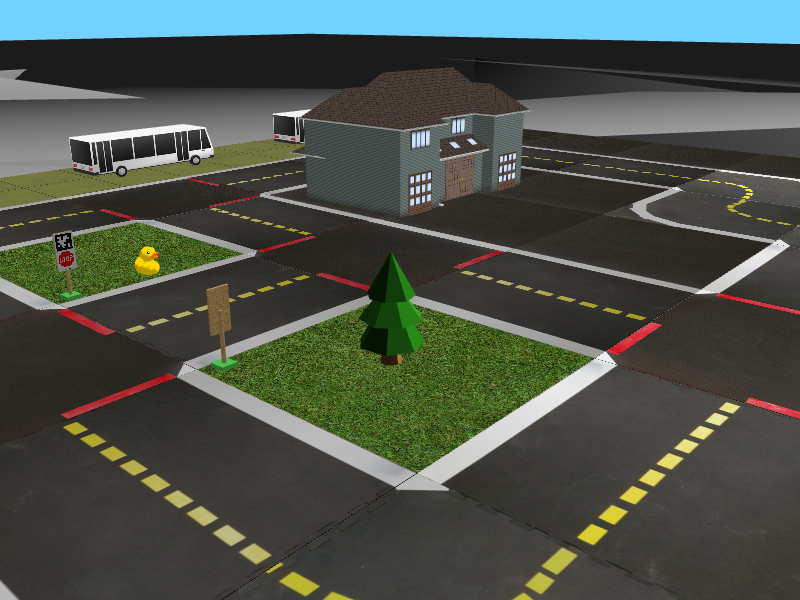
\includegraphics[width=0.6\textwidth]{kapitel2/images/duckietown-gym.png}
	\label{fig:duckietown-gym}
	\caption{Beispielhafte Darstellung des DuckieTown-Simulators}
	\vspace{0.2cm}
	\quelle\url{https://raw.githubusercontent.com/grusel-opi/gym-duckietown/master/media/simplesim_free.png}
\end{figure}

Der Simulator ist schnell, quelloffen und ausgesprochen anpassungsfähig. Er wurde zunächst für die einfache Linienverfolgung konzipiert und wurde dann im Laufe der Zeit zu einem voll funktionsfähigen Simulator für autonom fahrende Fahrzeuge, insbesondere im Bezug zur künstlichen Intelligenz. \cite{gym_duckietown}

